\chapter{Tecniche di spam detection}
Il capitolo illustra alcune tecniche di spam detection presenti in letteratura. Le tecniche verranno suddivise sulla base del tipo di segnali che vengono utilizzati, come: il contenuto, il grafo ottenuto dalla fase di crawling ed altri segnali (es. header delle richieste HTTP). Nella prima parte del capitolo verranno illustrate le tecniche basate sul contenuto, nella seconda parte le tecniche che fanno uso di grafi ed infine le tecniche che fanno uso di altri tipi di segnali.

\section{Tecniche basate sul contenuto}
\subsection{Periodo: 2004 - 2006}
Uno dei primi studi sul web spam è descritto in \cite{Fetterly:2004:SDS:1017074.1017077}, in questo articolo vengono eseguite delle analisi per confrontare alcune proprietà delle pagine spam e con contenuti in modo tale da estrarre dei valori tramite cui si può stimare se una pagina sia spam. Bisogna precisare che questi valori sono il risultato di studi empirici effettuati su alcuni dataset. Le proprietà vengono classificate come segue:
\begin{itemize}
 \item 	Proprietà degli URL. Come descritto in precedenza il \textit{link spam} è una forma di spam dove gli spammer cercano di aumentare il rank derivato dagli algoritmi basati sulla struttura dei link.Quindi uno spammer cerca di creare automaticamente tante pagine spam di bassa qualità che puntano a una pagina target \textit{p}. Alcune analisi sulle proprietà dei link mostrano che gli URL di un HOST sono buone feature per identificare lo spam. In particolare il nome di un HOST con molti caratteri, punti, barre e numeri è un buon indicatore di spam. Perciò un modo semplice per classificare le pagine sarebbe quello di usare un valore di soglia tale per cui superata tale soglia la pagina venga classificata come spam. 
 
 \item Host name resolution. Alcuni motori di ricerca (es. Google) data una query \textit{q}, calcolano un rank più alto a un URL \textit{u} se i termini che compongono  il nome dell'host di \textit{u} combaciano con i termini della query. Gli spammer per sfruttare questo meccanismo popolano gli URL delle pagine spam con termini contenuti in query molto frequentu che sono rilevanti per un certo settore.
 
 \item Proprietà del contenuto: le pagine generate automaticamente hanno tutte lo stesso template, ad esempio ci sono numerosi siti di spam che dinamicamente generano pagine che hanno uno stesso numero di parole. Una tecninca per determinare lo spam è quella di clusterizzare le pagine in base alla somiglianza dei template. Visto che le pagine di spam sono molto simili tra loro, identiicando molte pagine con la stessa struttura è probabile che siano di spam.
\end{itemize}

Oltre a queste proprietà base che servono per identificare lo spam in \cite{Ntoulas:2006:DSW:1135777.1135794}, un lavoro del 2006, vengono descritti una serie di metodi per l'indivuduazione dello spam. Ogni metodo è altamente parallelizabile, può essere eseguito in un tempo proporzionale alla dimensione della pagina e identifica lo spam di ogni pagina scaricata. Inolte questi metodi possono essere combinati con tecniche di machine learning per creare un algoritmo di rilevazione di spam più efficiente. Questo lavoro è un proseguio del lavoro precedentemente descitto \cite{Fetterly:2004:SDS:1017074.1017077}. In primis sono stati identificati quali domini e pagine (classidficate sulla base della lingua) contenesserò più spam. Il risultato ha evidenziato che i domini ``.biz, .us, e .com'' sono quelli con maggiore contenuto di spam mentre per quanto riguarda le pagine contententi più spam sono le francesi, tedesche e inglesi. I risultati sono rappresentati nei due grafici in figura \ref{fig:fetterly1} e in figura 
\ref{fig:fetterly2}. Questi risultati si basano sul dataset messo a disposizione degli autori che è stato ricavato utilizzando MSN Search crawler nell'agosto del 2004, per maggiori informazioni \cite{Ntoulas:2006:DSW:1135777.1135794}.
\begin{figure}[htbp]
\centering
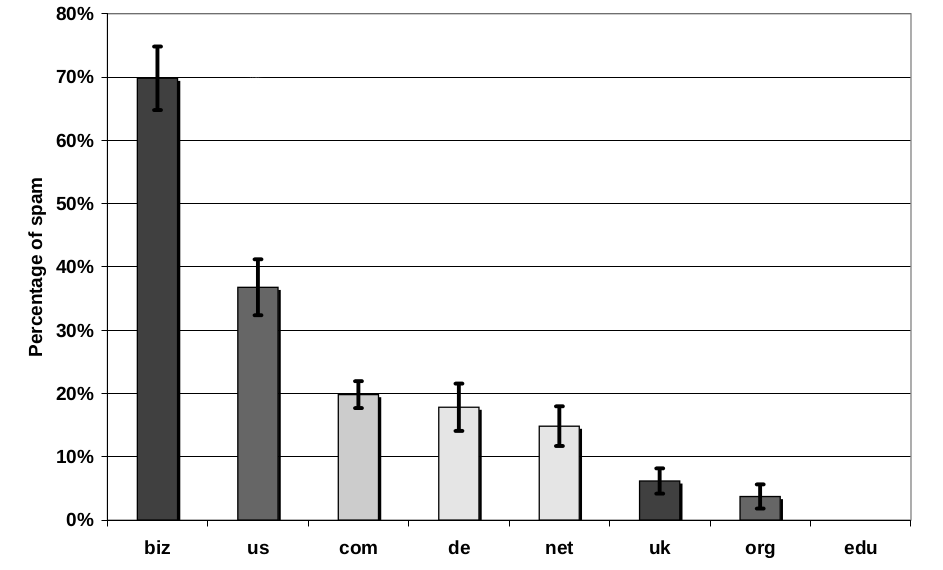
\includegraphics[width=12cm]{immagini/fetterly/fetterly1}
\caption{Occorrenze dello spam classificate per dominio all'iterno del dataset descritto in \cite{Ntoulas:2006:DSW:1135777.1135794}}
\label{fig:fetterly1}
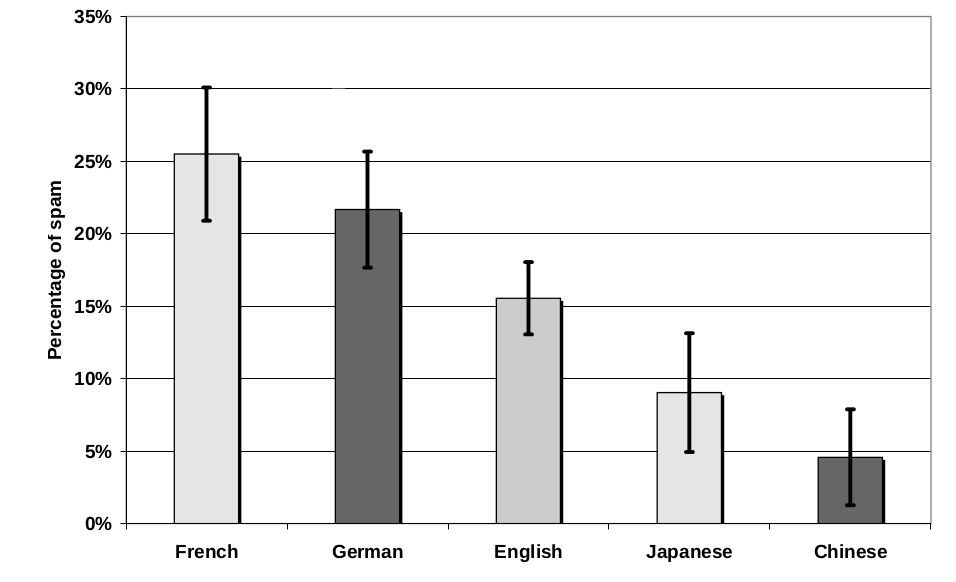
\includegraphics[width=12cm]{immagini/fetterly/fetterly2}
\caption{Occorrenze dello spam classificate per lingua all'iterno del dataset descritto in \cite{Ntoulas:2006:DSW:1135777.1135794}}
\label{fig:fetterly2}
\end{figure}

Una pratica molto comune nel costruire pagine spam è la cosidetta ``Keyword stuffing''. Durante questo processo il contentuto della pagina aumenta con un numero di parole popolari che sono irrilevanti con il resto della pagina. In molti casi per poter aumentare le probabilità di essere messa in cima al rank di molte query, il contenuto di una pagina spam viene aumentato con tante parole estrane all'argomento della pagina. In figura \ref{fig:fetterly3} viene plottato la distribuzione delle parole per ogni pagina del data set. Oltre alla distribuzione delle parole viene raffigurata la percentuale di pagine per ogni range di parole che sono considerate spam. Dal grafico viene notato che la prevalenza di spam è più alta nelle pagine con pmolte parole. Perciò c'è una correlazione tra prevalenza di spam e numero di parole. Il conteggio delle parole da solo non è una buona euristica visto che porta un alto tasso falsi positivi.
\begin{figure}[htbp]
\centering
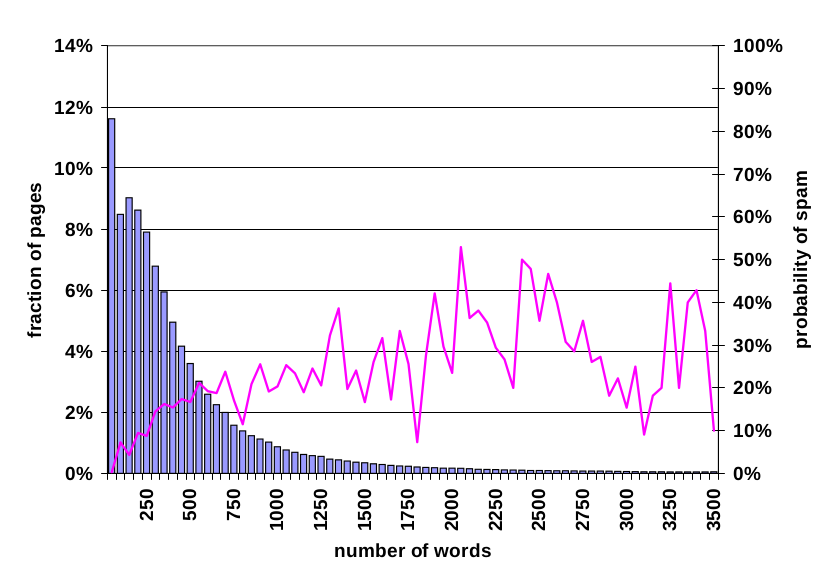
\includegraphics[width=12cm]{immagini/fetterly/fetterly3}
\caption{Prevalenza di spam sulla base del numero di parole per pagina}
\label{fig:fetterly3}
\end{figure}

La tecnica ``Keyword stuffing'' viene utilizzata anche per la costruzione dei titoli delle pagine spam dal momento che alcuni motori di ricerca assegnano un peso maggiore ai termini della query presenti all'interno del titolo della pagina. Il grafico in fugura \ref{fig:fetterly4} rappresenta la distribuzione del numero di parole all'interno dei titoli delle pagine. Come per gli altri grafici viene plottata la rispettiva percentuale di pagine spam. Dal grafico si vede che un'eccesso di parole all'interno del titolo è un indicatore (come per il contenuto della pagina) che una pagina è spam.
\begin{figure}[htbp]
\centering
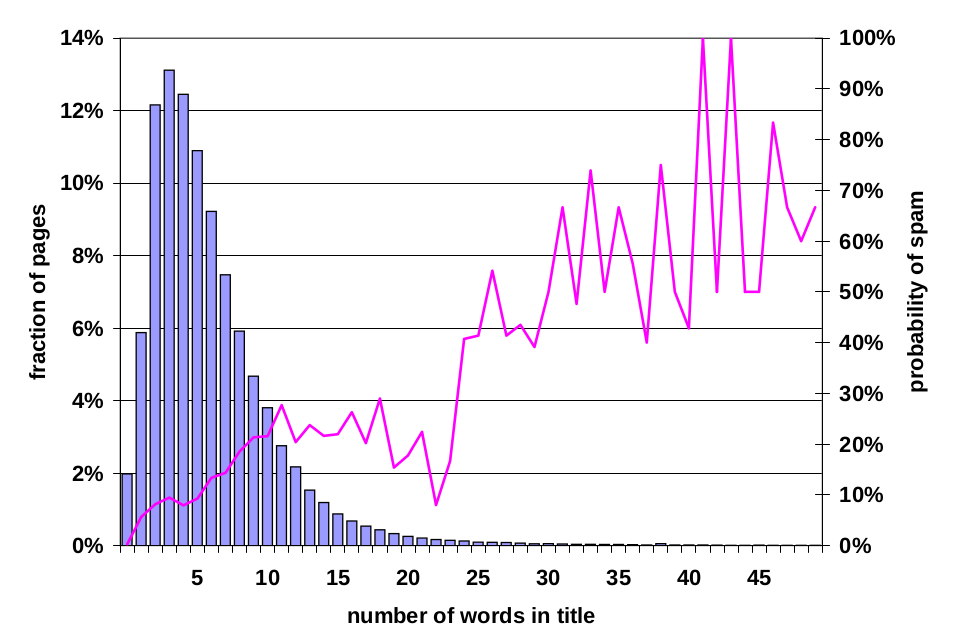
\includegraphics[width=12cm]{immagini/fetterly/fetterly4}
\caption{Prevalenza di spam sulla base del numero di parole all'interno dei titoli delle pagine}
\label{fig:fetterly4}
\end{figure}

Un altro dato trovato dagli autori per determinare se una pagina è spam riguarda la lunghezza media delle parole delle pagine. Dal dataset preso in considerazione in \cite{Ntoulas:2006:DSW:1135777.1135794} si nota che la distribuzione risultante della lunghezza media delle parole è simile a una gaussiana con moda e mediana corrispondenti a una media di 5.0. La maggior parte delle parole hanno una lunghezza media compresa tra 4.0 e 6.0. Come si nota dal grafico in figura \ref{fig:fetterly5} le parole con lunghezza media 10 sono certamente spam.
\begin{figure}[htbp]
\centering
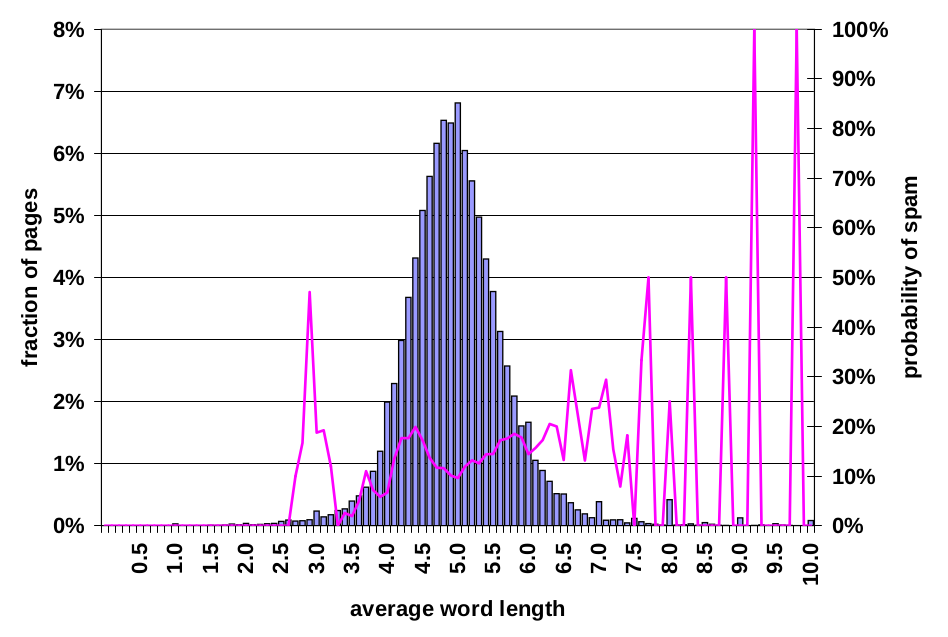
\includegraphics[width=12cm]{immagini/fetterly/fetterly5}
\caption{Prevalenza di spam sulla base della lunghezza media delle parole}
\label{fig:fetterly5}
\end{figure}